%%==================================================
%% chapter03.tex for TJU Master Thesis
%% Encoding: UTF-8
%%==================================================

\chapter{纤维编织层基本理论及有限元仿真方法}


\section{引~言}


\hacite 的理论模型正如第一章综述中介绍的,将加强层理论中的钢绞线理论,与复合材料的“特征单元”的研究思路结合。钢绞线理论本身就是为了加强层的大变形而被提出的,但对于编织加强层来说,该理论过度简化,编织结构的微结构特征,包括纤维的形状、曲线、分布等。引入“特征单元”后,就能很好的解决这个问题,同时相对复合材料的理论,能更容易地解决编织层“结构非线性”的问题。

可以理解为,\ha 理论模型是一种分析编织层微观结构,通过特征单元平均化(Homogenization),在宏观上能够反映编织层非线性力学性能的理论模型。事实上,\ha 并未深入挖掘该模型,提供的拉伸试验与仿真结构并不能在非线性段吻合。从仿真的角度来说,该模型不能直接应用于内压工况。

第二章详细介绍了软管组件的结构及重要参数,本章将 首先介绍\ha  的编织加强层理论,然后提出适用于该理论的有限元仿真方法。数值仿真的结果能结合试验,验证得到的本构模型是否合理。因此,对有限元建模的方法研究,也是本章的重内容之一。



\section{基本假设}
在对编织结构进行理论分析之前,首先需要明确几个基本的假设:

\begin{compactenum}[\bf 假设1  ]
	\item 编织层加强层中,纤维等周期均匀的分布在编织层所占据的空间中,即编织机编织过程稳定可靠,编织层个处得编织密度、编织角等参数保持一致;
	\item 编织层中的纤维不考虑由于相互接触挤压造成的直径变化;
	\item 纤维间间不发生相对滑动,编织角发生变化时,$ +\alpha$  、$-\alpha $两个方向的钢丝只绕着节点转动,节点如图\ref{fig:braid-angle-chap3-1}所示。
\end{compactenum}

实际上,编织加强层的工艺控制是比较困难的,这里假设编织层均匀,是采用“特征单元”分析的基础;不考虑纤维相对挤压的形变是为了简化模型分析的发杂程度;编织较为紧密时,以及纤维上下穿行的相互限制,纤维延纤维轴向滑动是很困难的。如图\ref{fig:hypothesis}所示,编织层拉伸后涂黑处仍能保持原来的特征,表明纤维间没有发生相对滑动。

	
	\begin{figure}[!htp]
\centering
\subfigure{
	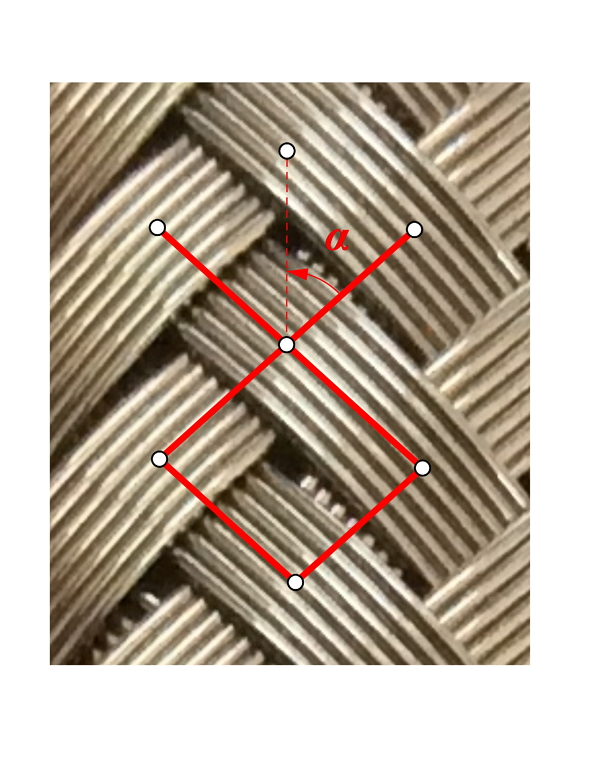
\includegraphics[height=0.2\textheight]{figure/chap2/braid-angle}
	}
\subfigure{
	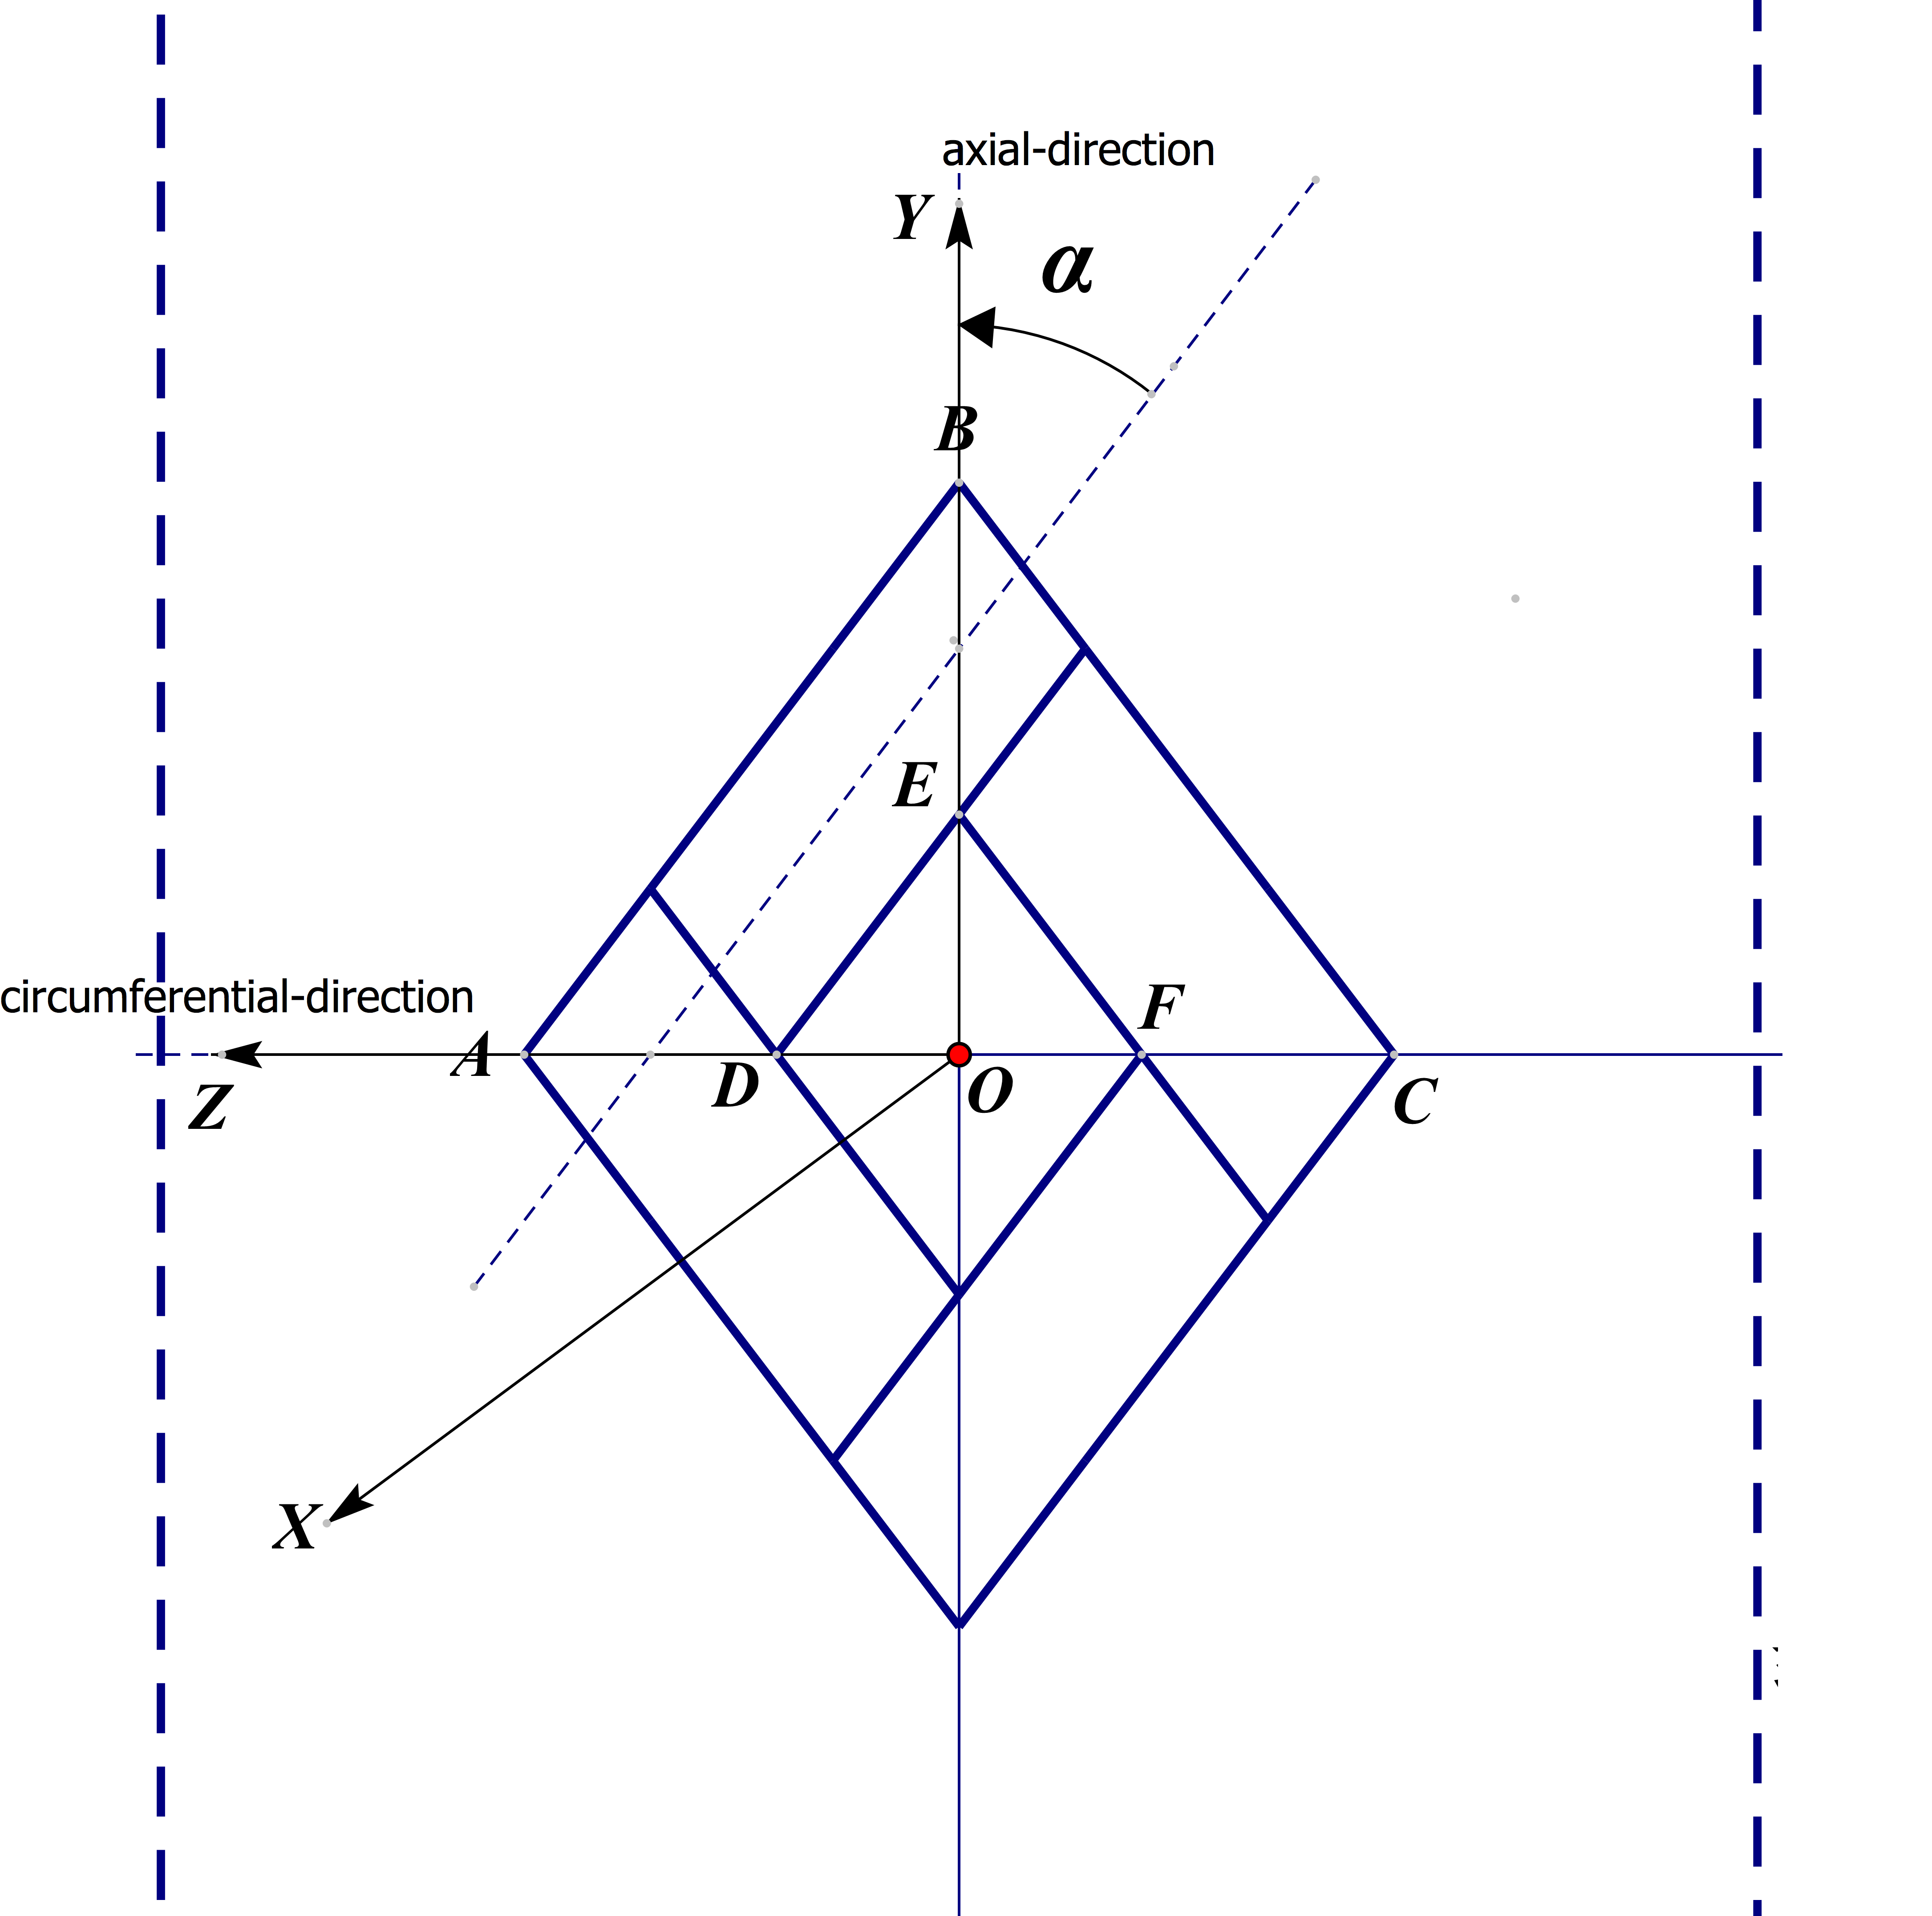
\includegraphics[height=0.2\textheight]{figure/chap2/braid-angle-2}
	}
\subfigure{
	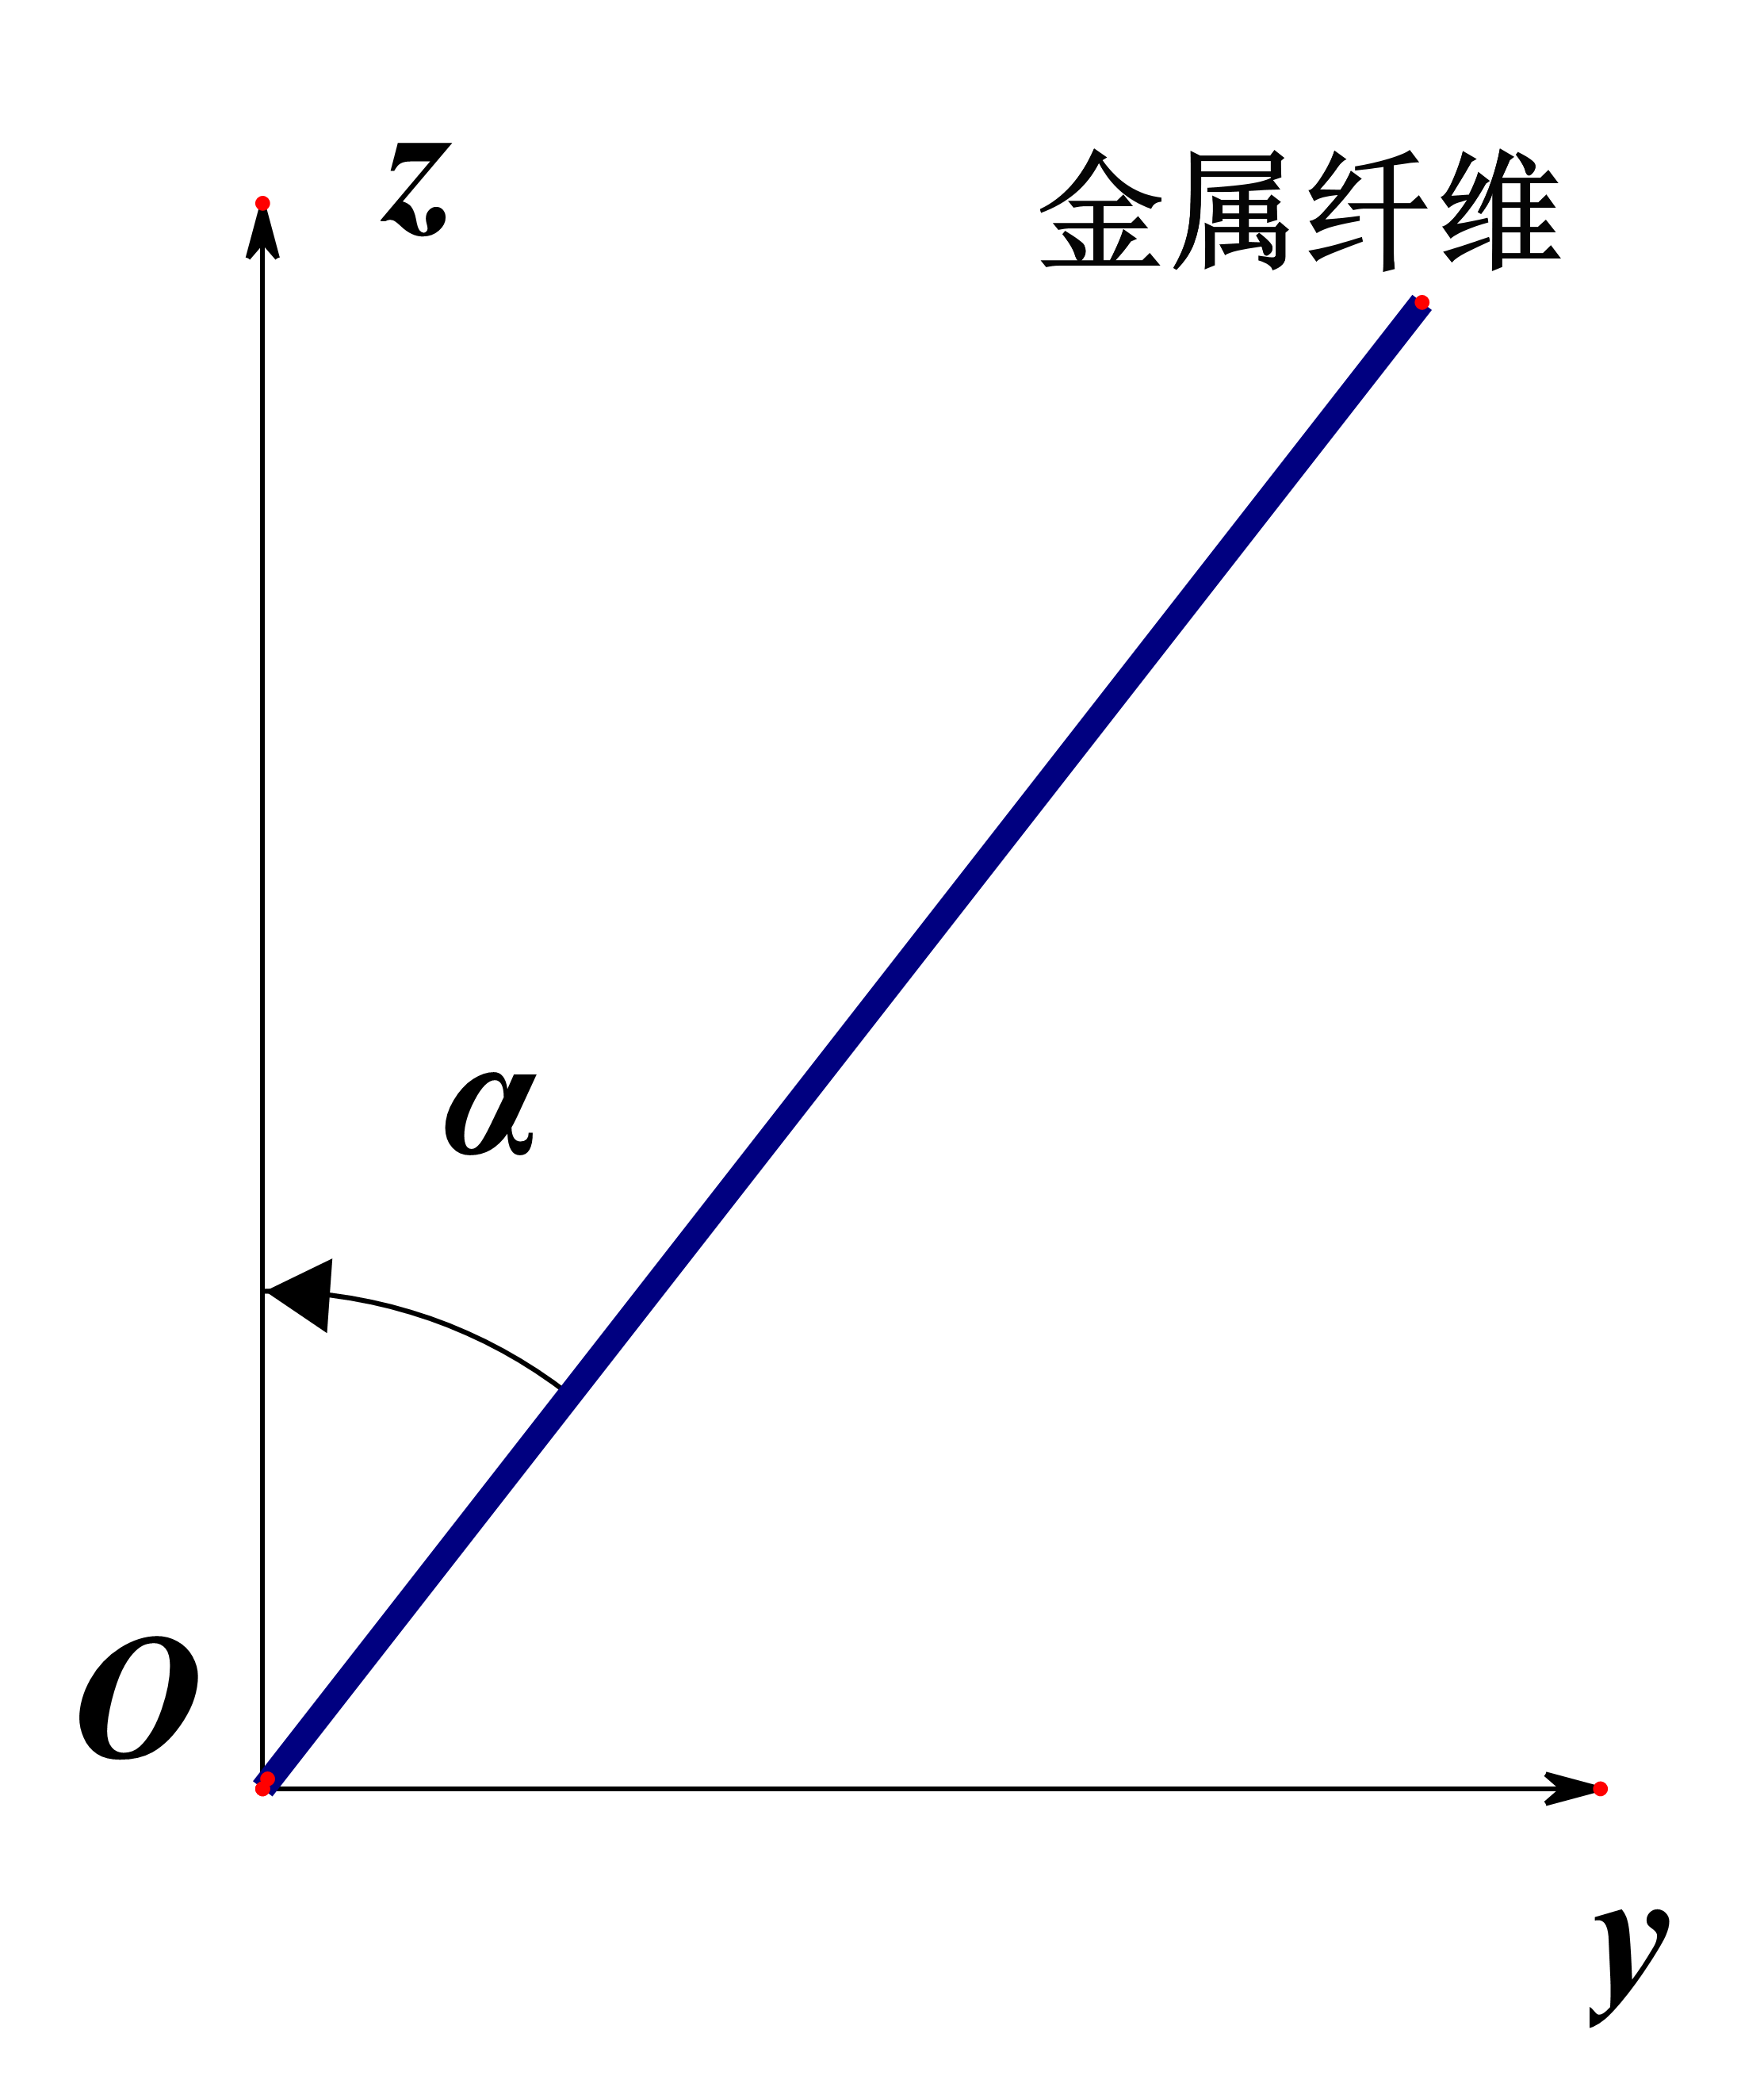
\includegraphics[height=0.2\textheight]{figure/chap2/braid-angle-3}
	}
\fcaption{编织角的定义}{Definition of braid angle}
\label{fig:braid-angle-chap3-1}
\end{figure}

\begin{figure*}[!htp]
	\centering
	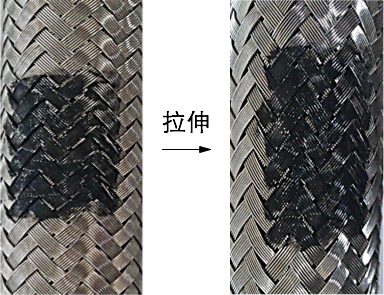
\includegraphics[width=0.5\linewidth]{figure/chap3/hypothesis}
	\fcaption{验证纤维间不相对滑动假设}{}[纤维不滑动假设]
	\label{fig:hypothesis}
\end{figure*}

\section{基本理论}

编织加强层的本构理论可以分为两个部分:1、刚度矩阵;2、编织角。编织层的刚度矩阵由编织角确定。而软管轴向受拉时,编织角会相应发生改变,则编织层的刚度也会发生改变,两者相互偶合。


\subsection{确定特征单元}
首先要去顶编织ceng层的特征单元,如图\ref{fig:unit},为编织层中周期性出现的单元,根据假设3,纤维间间不发生相对滑动,编织角发生变化时,纤维除了自身弹性伸长外,只绕着节点转动。将节点间的纤维抽象为杆单元(bar element),即为基本的特征单元。
\begin{figure*}[!htp]
\centering
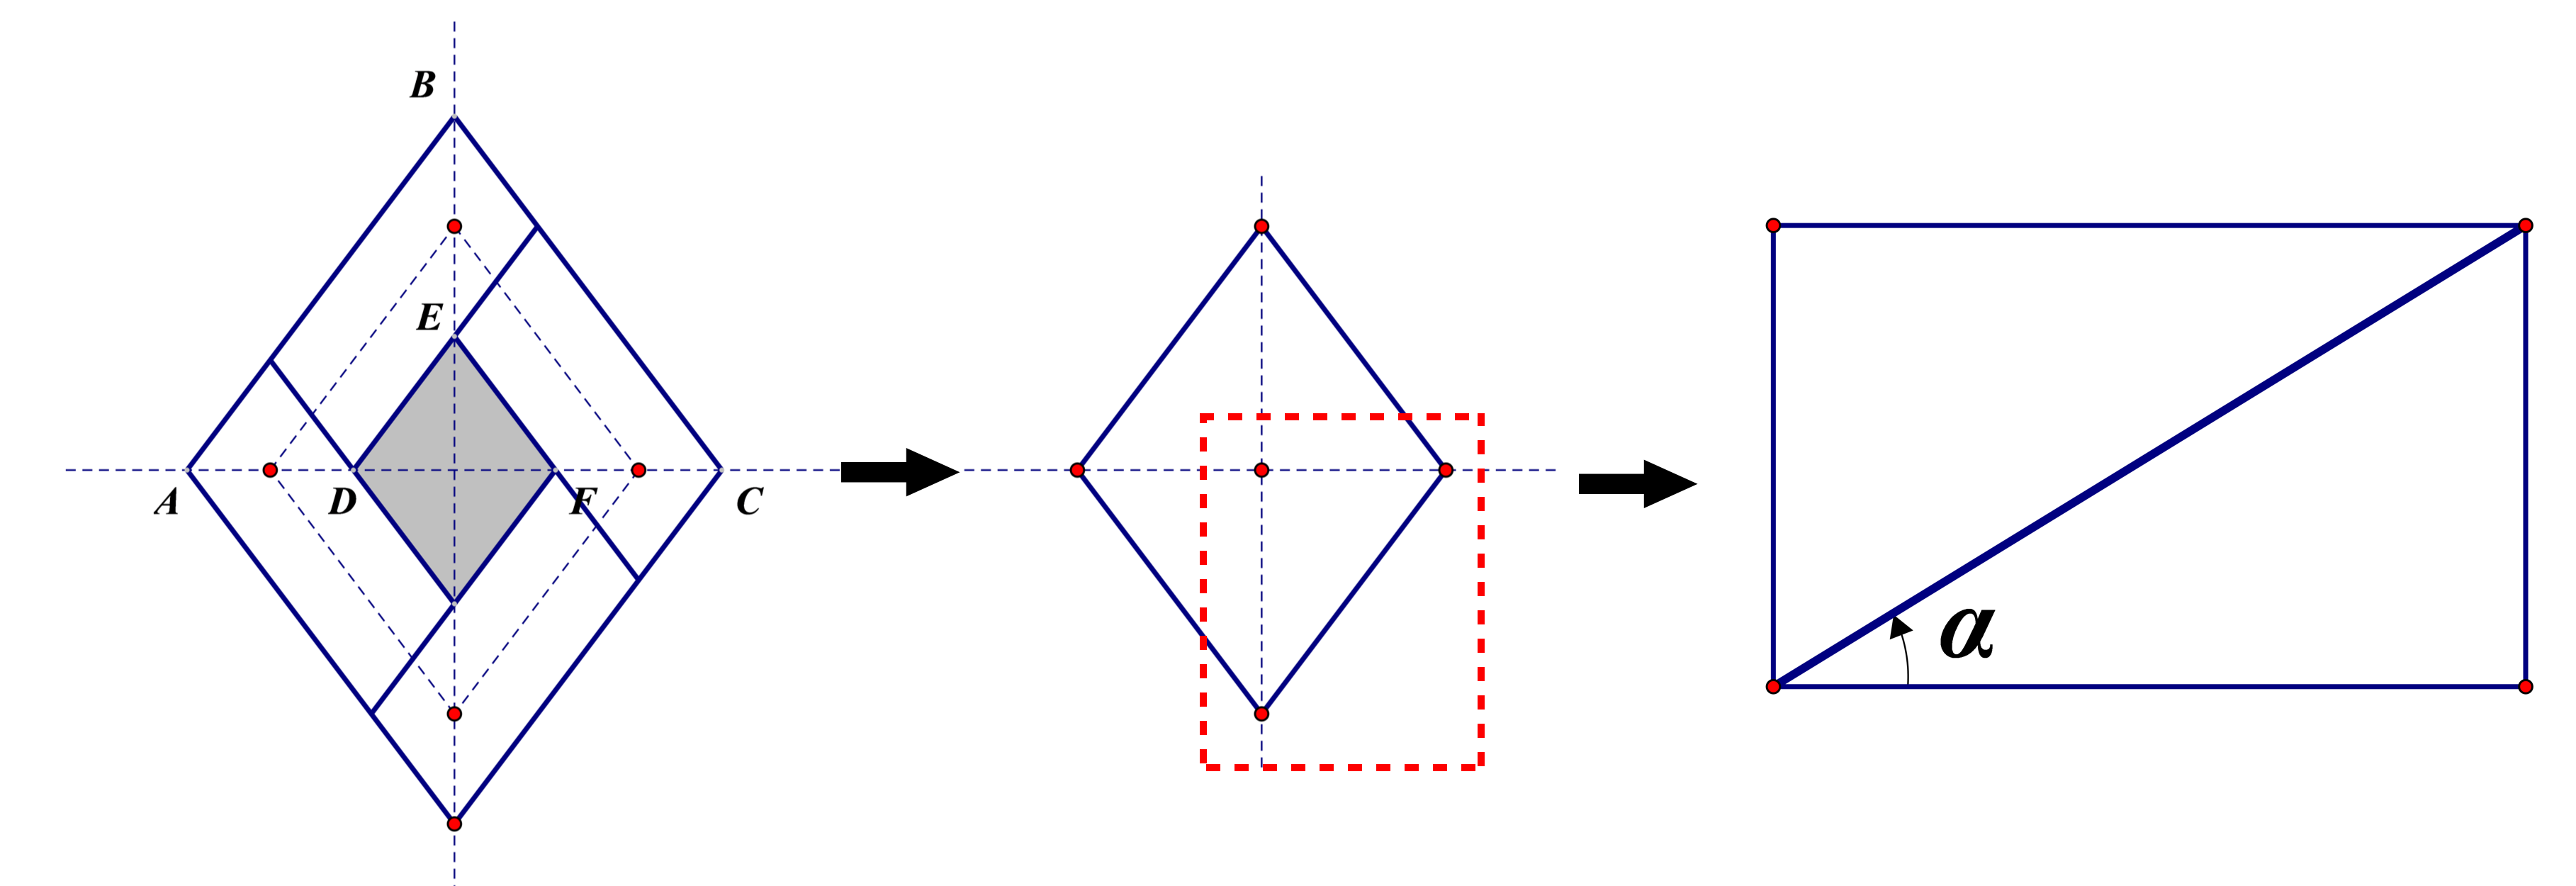
\includegraphics[width=0.9\linewidth]{figure/chap3/unit}
\fcaption{确定基本特征单元}{definition of representative unit cell}
\label{fig:unit}
\end{figure*}




\subsection{基本刚度矩阵}
首先确定单层螺旋缠绕的刚度矩阵:取一个代表性体积单元,
其在平面内的宏观应变为
$ {\varepsilon _{ij}}\left( {i,j = 2,3} \right)$ ,
根据基本假设各股金属纤维之间不发生相对滑动,可以认为金属纤维与特征单元变形协调,则方向为$  \vec{n} $的金属纤维向$ \lambda_f $应变为\cite{gaosiyang2009}:







\begin{equation}
{\lambda _f} = {\varepsilon _{ij}}{n_i}{n_j}
\end{equation}

其中,$ n_i\left( {i,j = 2,3} \right) $为金属纤维取向的方向余弦:

\begin{equation}
\label{eq:fiber-strain}
\left\{ {\begin{array}{*{20}{c}}
	{{n_1} = \cos \alpha }\\
	{{n_2} = \sin \alpha }
	\end{array}} \right.
\end{equation}

$ E $为金属纤维弹性模量,则该去向金属纤维的应变能密度可以表示为:

\begin{equation}
{{W_f} = \int E {\lambda _f}d{\lambda _f} = \frac{1}{2}\sum {E{{\left( {{\lambda _f}} \right)}^2}} {V_f}}
\end{equation}

代入\ref{eq:fiber-strain}式,可得

\begin{equation}
{{W_f} = \frac{1}{2}\sum {E \cdot {n_i}{n_j}{n_k}{n_l}{\varepsilon _{ij}}{\varepsilon _{kl}}}  \cdot {V_f}\left( {i,j,k,l = 1,2} \right)}
\end{equation}

则单层金属纤维螺旋缠绕的宏观刚度张量为:

\begin{equation}
{{C_{f,ijkl}} = \frac{{{\partial ^2}{W_f}}}{{\partial {\varepsilon _{ij}}\partial {\varepsilon _{kl}}}} = \xi E \cdot {n_i}{n_j}{n_k}{n_l}}
\end{equation}
矩阵形式为:
\begin{equation}\small
{\hangjut{1}
C_{ijkl}^{helix} = \left[ {\begin{array}{*{20}{c}}
	{\rm{0}}&{\rm{0}}&{\rm{0}}&{\rm{0}}&{\rm{0}}&{\rm{0}}\\
	{\rm{0}}&{\xi E \cdot {{\cos }^4}\alpha }&{\xi E \cdot {{\cos }^2}\alpha {{\sin }^2}\alpha }&0&{\rm{0}}&{\xi E \cdot {{\cos }^3}\alpha \sin \alpha }\\
	{\rm{0}}&{\xi E \cdot {{\sin }^2}\alpha {{\cos }^2}\alpha }&{\xi E \cdot {{\sin }^4}\alpha }&0&{\rm{0}}&{\xi E \cdot \cos \alpha {{\sin }^3}\alpha }\\
	{\rm{0}}&{\rm{0}}&{\rm{0}}&{\rm{0}}&{\rm{0}}&{\rm{0}}\\
	{\rm{0}}&{\rm{0}}&{\rm{0}}&{\rm{0}}&{\rm{0}}&{\rm{0}}\\
	{\rm{0}}&{\xi E \cdot {{\cos }^3}\alpha \sin \alpha }&{\xi E \cdot \cos \alpha {{\sin }^3}\alpha }&{\rm{0}}&{\rm{0}}&{\xi E \cdot {{\sin }^2}\alpha {{\cos }^2}\alpha }
	\end{array}} \right]
}
\end{equation}

其中,$  \xi $为覆盖系数,叠加两层编织角分别为$  + \alpha  $ , $- \alpha  $ 的缠绕层的刚度矩阵,即可得到相应编织层的刚度矩阵,
\begin{equation}\small
{\hangjut{1}
C_{ijkl}^{braid} = \left[ {\begin{array}{*{20}{c}}
	{\rm{0}}&{\rm{0}}&{\rm{0}}&{\rm{0}}&{\rm{0}}&{\rm{0}}\\
	{\rm{0}}&{2\xi E \cdot {{\cos }^4}\alpha }&{2\xi E \cdot {{\cos }^2}\alpha {{\sin }^2}\alpha }&0&{\rm{0}}&{\rm{0}}\\
	{\rm{0}}&{2\xi E \cdot {{\sin }^2}\alpha {{\cos }^2}\alpha }&{2\xi E \cdot {{\sin }^4}\alpha }&0&{\rm{0}}&{\rm{0}}\\
	{\rm{0}}&{\rm{0}}&{\rm{0}}&{\rm{0}}&{\rm{0}}&{\rm{0}}\\
	{\rm{0}}&{\rm{0}}&{\rm{0}}&{\rm{0}}&{\rm{0}}&{\rm{0}}\\
	{\rm{0}}&0&0&{\rm{0}}&{\rm{0}}&{2\xi E \cdot {{\sin }^2}\alpha {{\cos }^2}\alpha }
	\end{array}} \right]
}
\end{equation}


\subsection{基础编织角理论}

特征单元得到轴向应变$  \varepsilon_{22} $与编织角的关系

\begin{figure*}[!htp]
	\centering
	\subfigure[]{
		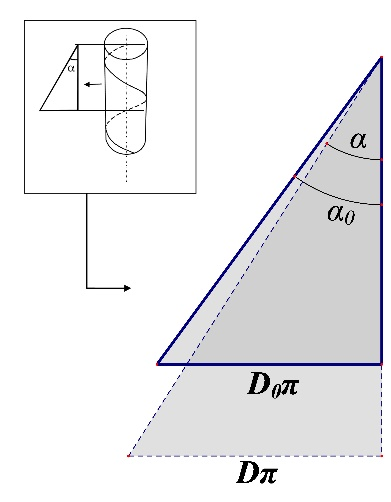
\includegraphics[height=0.25\textheight]{figure/chap5/unit-cell-2}}
	\hspace{0.5cm}
	\subfigure[]{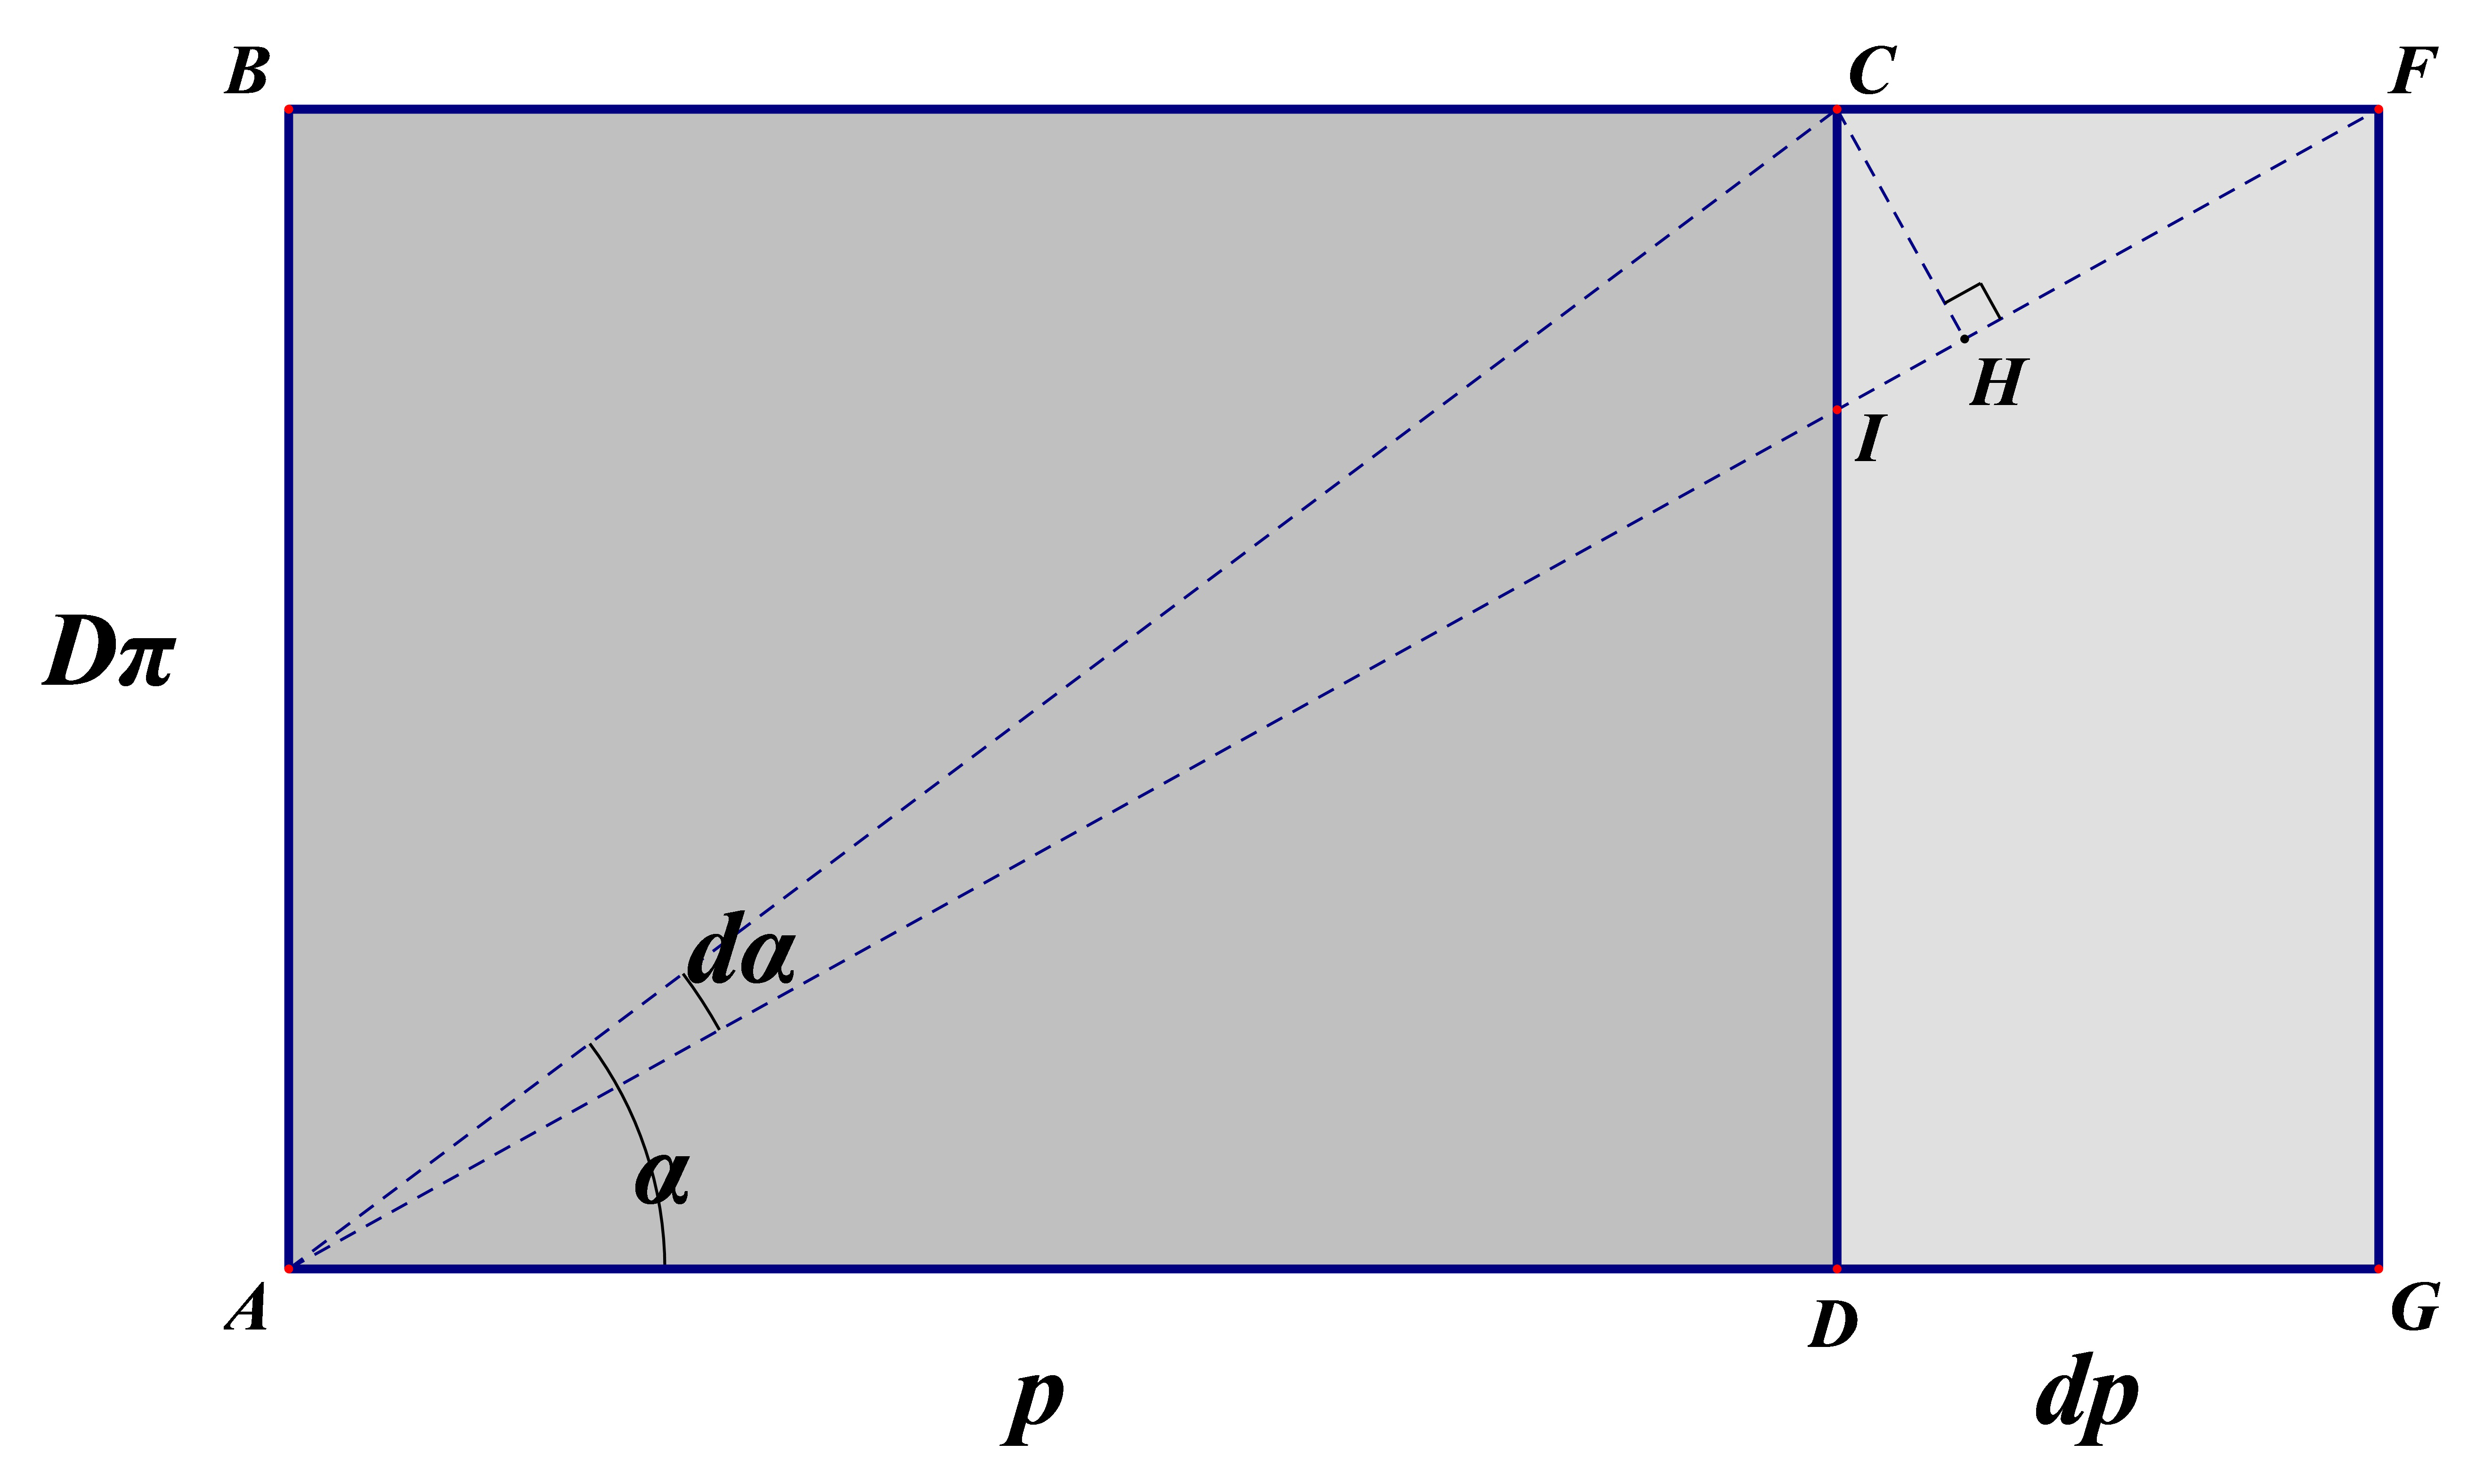
\includegraphics[height=0.2\textheight]{figure/chap5/unit-cell-1}}
	\fcaption{基本理论特征单元}{basic representative unit cell}
	\label{fig:unit-cell-2}
\end{figure*}

根据特征单元编织角变化的几何关系,可得
\begin{equation}
d\alpha  = \frac{{{\varepsilon _{22}}\sin \alpha \cos \alpha }}{{1 + {\varepsilon _{22}}{{\cos }^2}\alpha }}_{}
\end{equation}
其中, $ \varepsilon_22= dp/p $。特征单元纤维伸长量$ \varepsilon_f $,


\begin{equation}
{\varepsilon _f} = \sqrt {\frac{{{{\left( {{\varepsilon _{22}} + 1} \right)}^2} + \tan {\alpha ^2}}}{{1 + \tan {\alpha ^2}}}}  - 1
\end{equation}

编织加强层受到荷载后长度$ L $与直径$ D $都会发生相应的变化,根据钢绞线理论可以得到编织层初始长度、直径、编织角与加载后长度$ {L_0} $、直径$ {D_0} $与编织角$ {\alpha _0} $间的关系。
\begin{equation}
D = {D_0}\frac{{\sin \left( {\frac{\beta }{2}} \right)}}{{\sin \left( {\frac{{{\beta _0}}}{2}} \right)}} = D\frac{{\sin \left( \alpha  \right)}}{{\sin \left( {{\alpha _0}} \right)}}
\end{equation}

\begin{equation}
L = {L_0}\frac{{\cos \left( {\frac{\beta }{2}} \right)}}{{\cos \left( {\frac{{{\beta _0}}}{2}} \right)}} = {L_0}\frac{{\cos \left( \alpha  \right)}}{{\cos \left( {{\alpha _0}} \right)}}
\end{equation}


\subsection{编织角锁定假设}

\hacite 对软管组件进行了拉伸试验,同时根据其理论模型给出了数值仿真计算结果,对比拉伸试验的力位移曲线,如\ref{fig:hachemi-chap3}所示,

\begin{figure}[!htp]
	\centering
	\subfigure[]{
		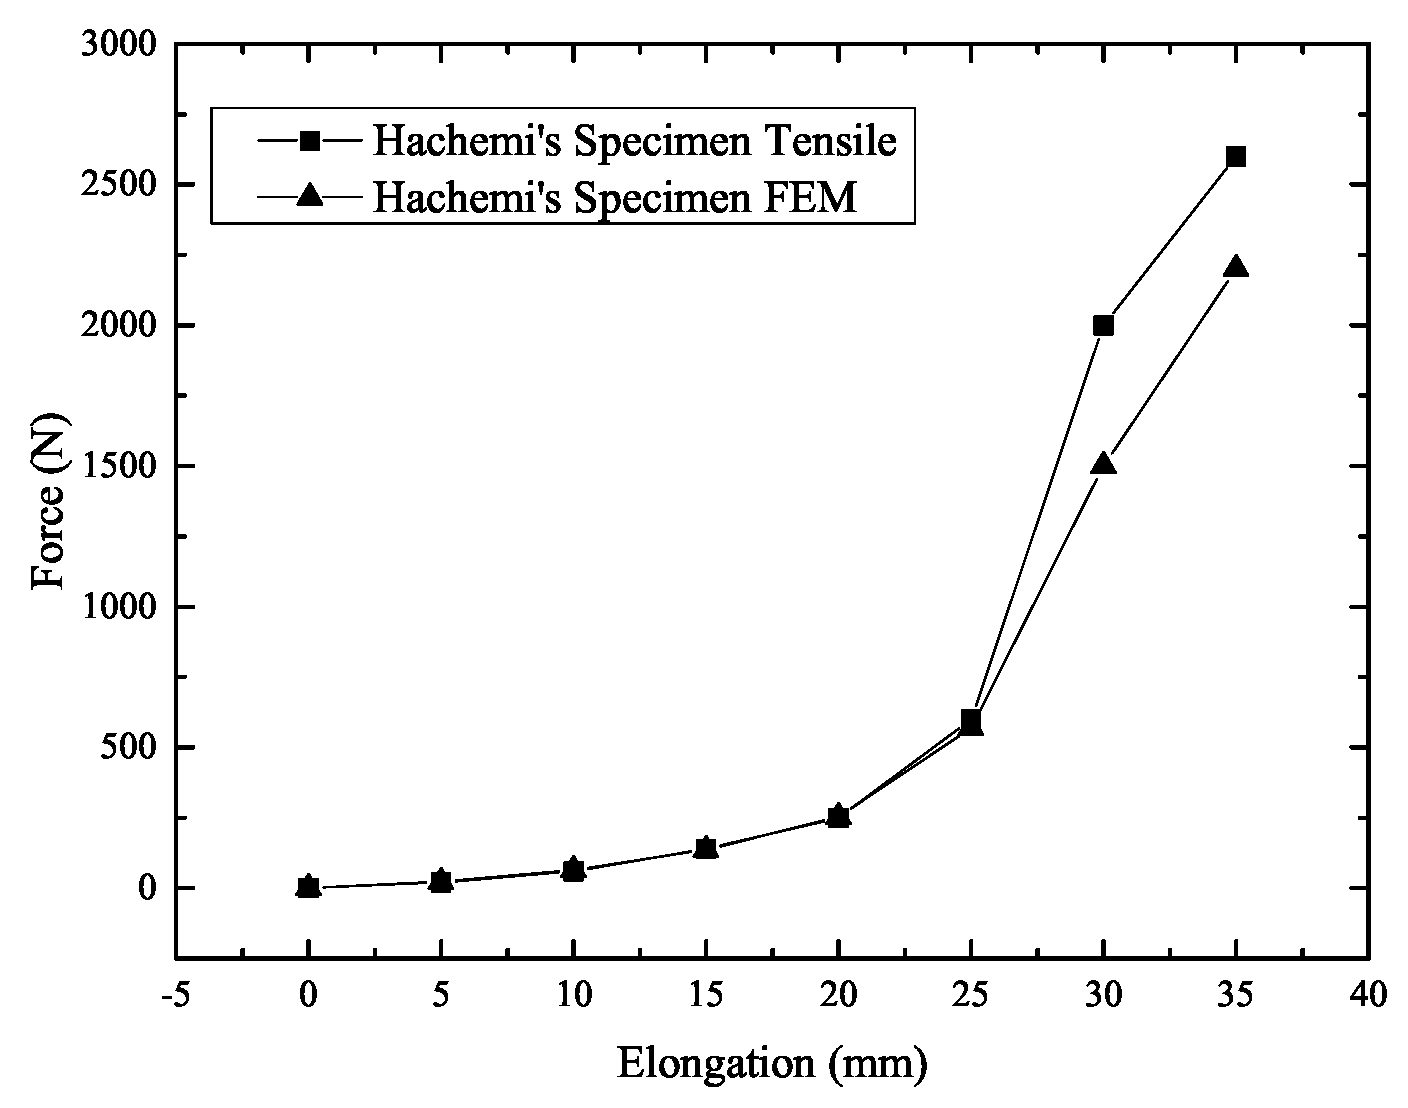
\includegraphics[height=0.2\textheight]{figure/chap1/hachemi}
		\label{fig:hachemi-chap3}
	}
	\hspace{1cm}
	\subfigure[]{
		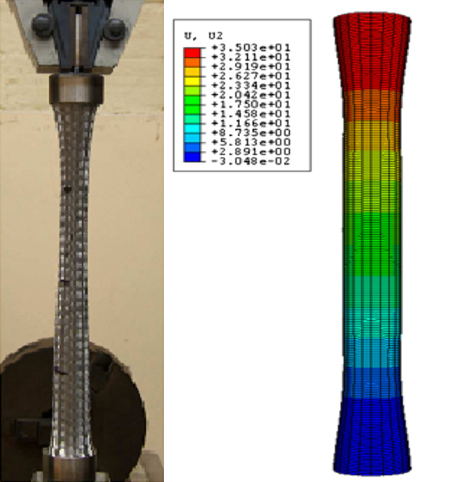
\includegraphics[height=0.19\textheight]{figure/chap1/hachemi-test}
		\label{fig:hachemi-test-chap3}
	}
	\subfigure[]{
		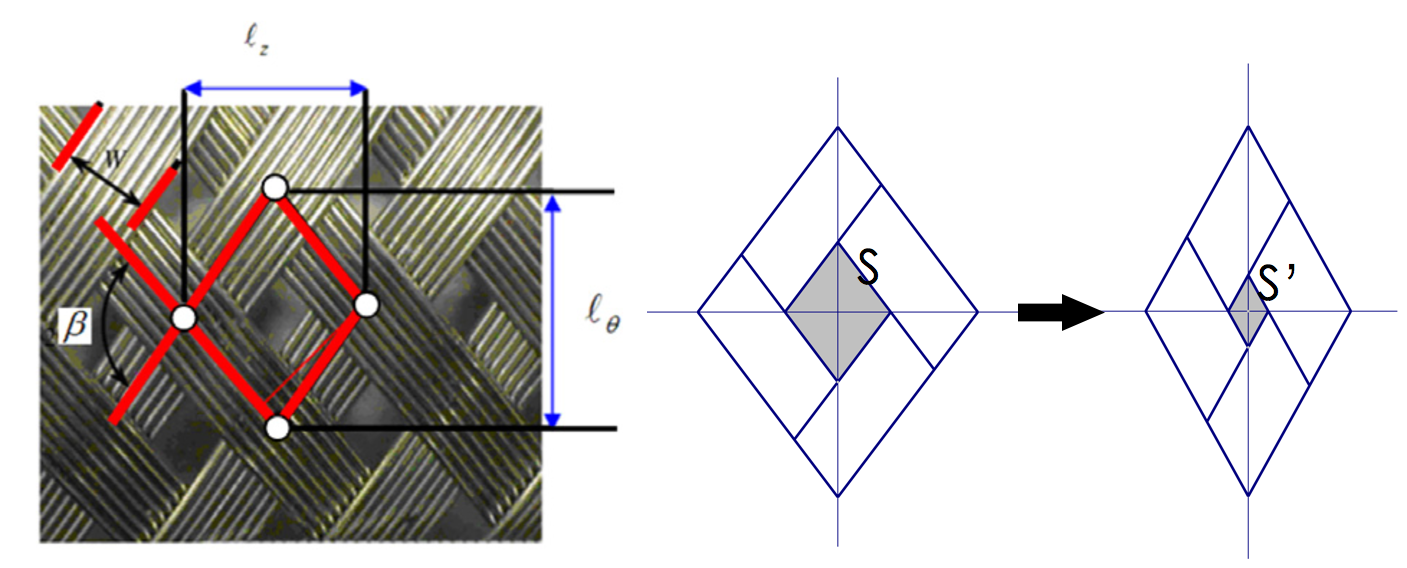
\includegraphics[width=0.7\linewidth]{figure/chap3/lock-hypo}
		\label{fig:gap-lockgap-lock}
	}
	
	\fcaption{\ha 拉伸试验}{\ha tensile experiment}
\end{figure}

尽管力位移曲线整体趋势一致,但在非线性段并不能很好的吻合。\ha 给出了编织角锁定假设来解释这一现象。编织层纤维间的空隙面积为$ S $(如图\ref{fig:gap-lockgap-lock}所示),当$ S = 0 $时,可以求得锁定编织角$ \alpha_c $:

\begin{equation}
\label{eq:lockalpha}
{\alpha _c} = \frac{1}{2} \cdot \arcsin \left( {\frac{W}{l}} \right)
\end{equation}

其中,$ W $为一股纤维的宽度,$ l  $为特征单元沿纤维方向的长度。
以上为\ha 模型的基本内容。





\section{编织加强层有限元仿真方法}

研究编织层本构的很大一部分目的是为了能够利用有限元软件对软管组件进行数值仿真试验,以减小编织层设计阶段对试验的依赖。同时,数值仿真的结果也能结合试验,验证得到的本构模型是否合理。因此数值仿真也是本研究的重点内容之一。

本研究有限元仿真采用的是通用有限元软件\aba ,因其具备较强的用户二次开发本构关系的接口。下面对\aba 软件进行简要的介绍。


\subsection{\aba 软件及\uma 介绍}
    ABAQUS由美国HKS公司研制开发,是目前世界上最流行、最先进、功能
最强大的大型通用商业有限元软件之一。ABAQUS自1997年进入我国以来就受到极大地关注,越来越多的国内高校、科研单位以及企业采用它作为科学研究和产品研发的工具。


ABAQUS可以进行结构静力、动力分析,拥有丰富的材料模型库、单元库
以及良好的扩展功能,能够模拟各种常见工程材料的性能,如金属、钢筋混凝土、土壤、岩石、橡胶、高分子材料、复合材料和可压缩超弹性泡沫材料等。同时,ABAQUs具有强大的非线性计算能力,可以进行几何非线性计算。ABAQUS/Standard在计算几何非线性问题时,采用的正是U.L.法。对于实体单元来说,无论采用内置的还是用户自定义的本构模型,ABAQUS/Standard均采用Jaumann应力率。


    ABAQUS为了方便和鼓励用户开发自己研究或感兴趣的材料模型,通过
FORTRAN语言接口,为用户提供了若干用户子程序(User Subroutines)和在编程时可以调用的实用程序(Utility Routines),以便用户自行定义符合自己所研究问题的模型。在ABAQUS提供的用户子程序中,与开发用户自定义材料的本构模型直接相关的是\uma 。通过ABAQUS主求解程序的接口,\uma 可以实现与ABAQUS的数据交流。
    \uma 的功能非常强大,使用\uma 子程序可实现下列功能\cite{lijinzhu2011}:
 \begin{compactenum}
\item 定义ABAQUS材料库中没有包含的材料的本构模型,进行有限元计算,
 	    以扩充程序功能。
\item 用于包含力学行为的任意分析过程将用户自定义的材料属性赋给
 	    ABAQUS计算模型中的任何单元。
\item 在计算中定义、使用、输出与求解相关的状态变量(Solution Dependent
 	    Variable,简称SDV ),便于追踪计算过程。
\item 可以和多个用户子程序如USDFLD. \uma HT等)联合使用,并且
 	    共享SDV空间。
 \end{compactenum}

\subsection{\uma 实现方法}

按照\aba 用户一子程序的约定,\uma 子程序需要定义单元积分点的材料刚度系数矩阵( Jacobian矩阵),并完成应力、应变以及求解状态变量的更新。
调用UMAT用户子程序进行分析的流程如图\ref{fig:umat-diaoyong}所示。
\begin{figure*}[!htp]
	\centering
	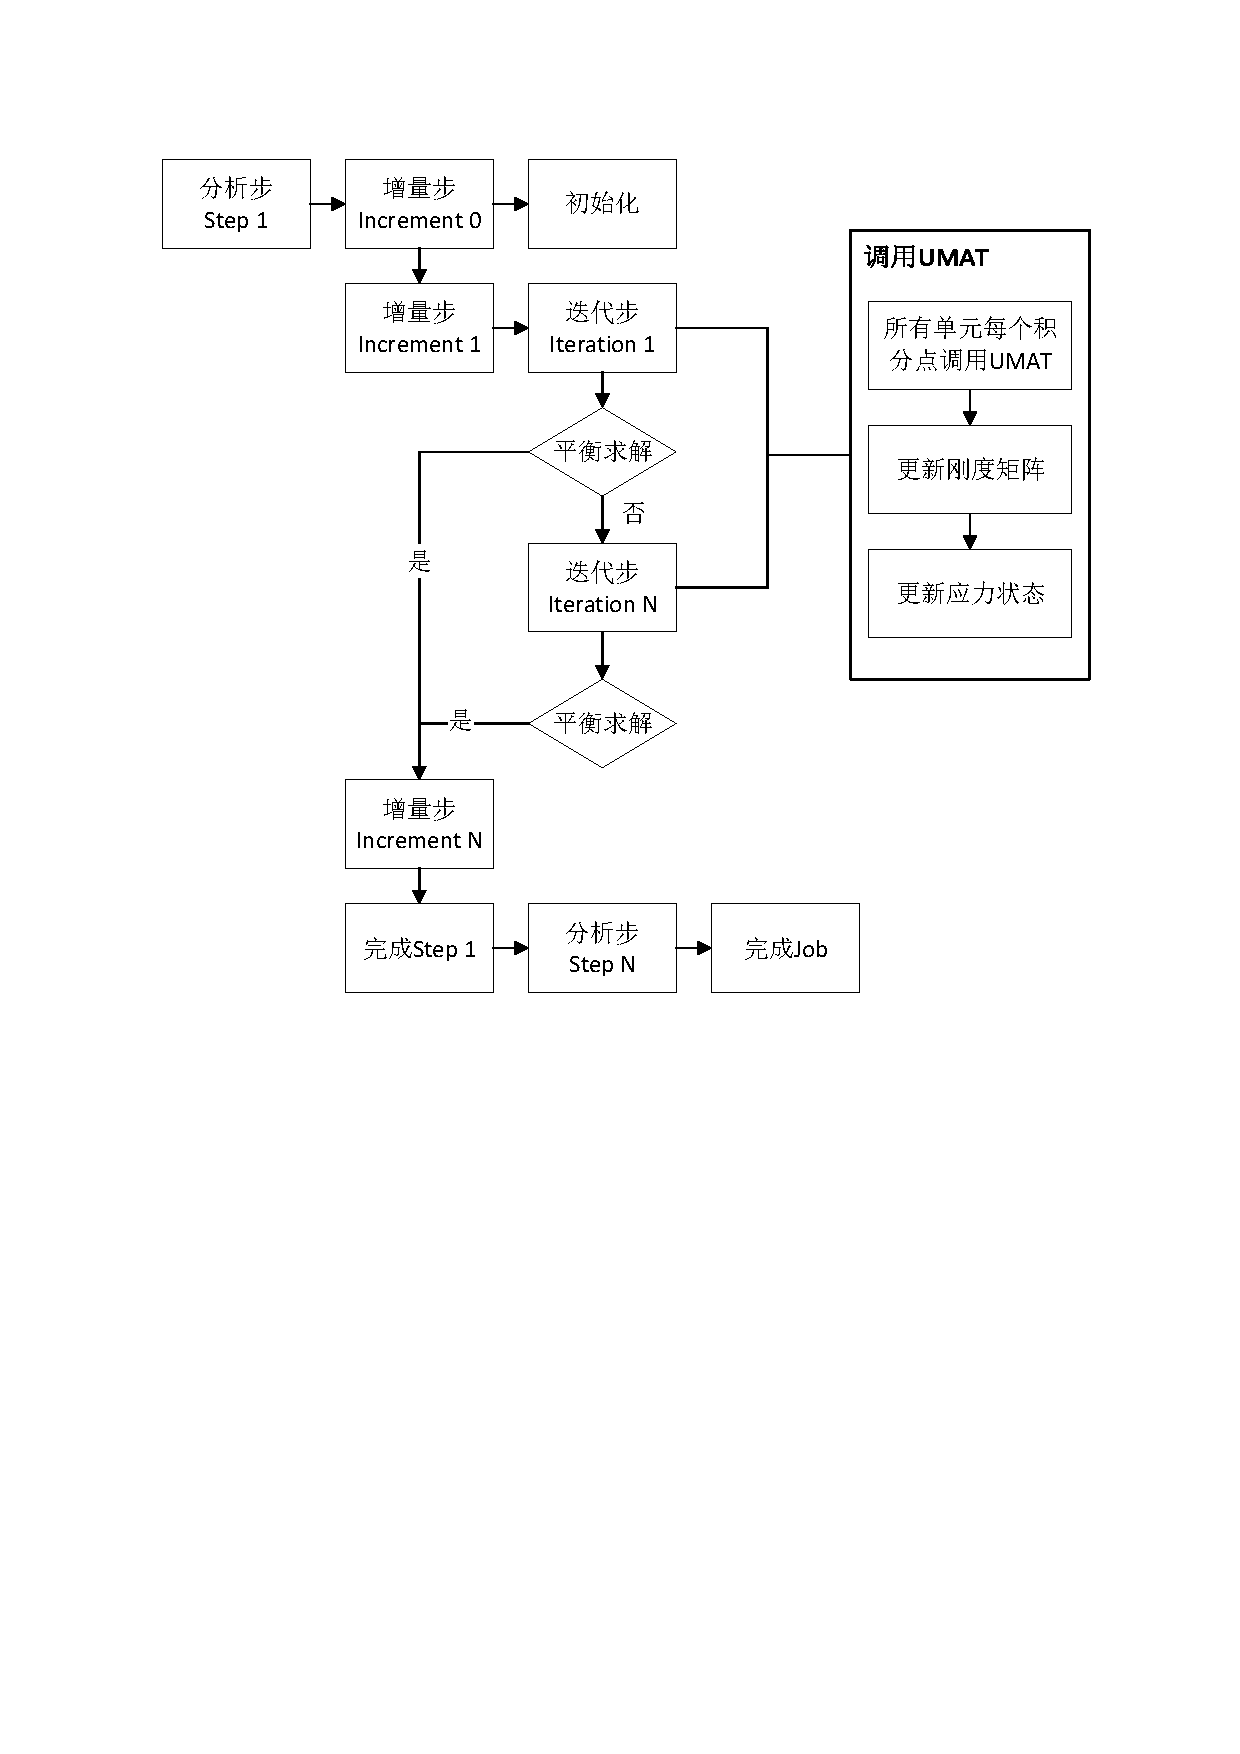
\includegraphics[width=0.7\linewidth]{figure/chap3/umat-diaoyong}
	\fcaption{调用UMAT用户子程序流程}{}
	\label{fig:umat-diaoyong}
\end{figure*}


根据ABAQUS的非线性增量加载方法与平衡迭代求解方法。ABAQUS如果在运行过程中发现用户子程序\uma 的存在,它将在每一个增量加载步初始时刻,在模型的每一个计算单元中的材料积分点上调用用户子程序UMAT,并根据用户程序代码计算刚度系数矩阵$ \bm{D} $,然后形成刚度矩阵一$ \bm{K} $,并由刚度矩阵$ \bm{K} $和当前增量步的荷载增量$ \bm{\Delta R} $ 求解位移增量$ \bm{\Delta U} $,然后进行平衡校核。如果平衡校核不满足默认误差或用户指定的误差,\aba 将继续进行平衡迭代,直到达到收敛要求,然后进入下一增量步的求解。

\aba 的用户子程序主体结构至少应包括以下六个部分:
\begin{inparaenum}[(1)]
\item ABAQUS约定的子程序题名说明;
\item  ABAQUS定义的参数说明表;
\item 开发者定义的局部变量说明表;
\item 开发者编写的程序代码段;
\item 子程序返回语句;
\item 结束语句。
\end{inparaenum}   


%\subsection{编织层算例}
%
\subsection{模型建立}

建立有限元建模的方法体系,适当简化模型,使得在保证计算精度的情况下, 提高运算效率;同时适当的简化,合理的建模方法也是计算精度的保证,避免了 机器误差在计算工程中累积。

由于软管组件与接头的接触非常复杂(如图\ref{fig:coupling}所示),但不会对拉伸试验的仿真有很大的影响。证 据是,试验中的金属纤维层一般在接头处发生脆断(见第四章内容),而非逐渐拉脱。因此几何模型需要对接头进行简化,以减少计算量。如图\ref{fig:periodic-sym-2}所示,可以采用固支的边界条件简化接头,并进一步采用周期对称的手段简化拉伸试验的有限元模型,如图\ref{fig:periodic-sym-3}所示。


\begin{figure*}[!htp]
\centering
\subfigure[接头几何模型]{
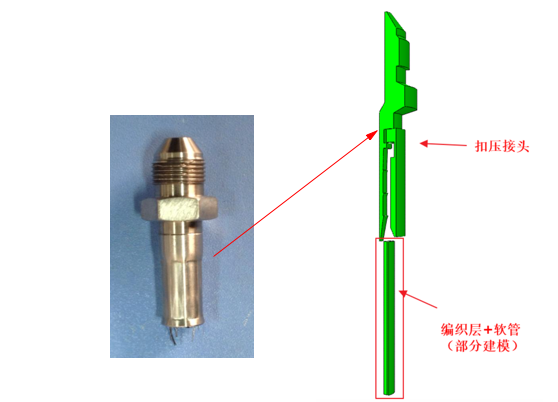
\includegraphics[width=0.4\linewidth]{figure/chap3/FEM/coupling}\label{fig:coupling}
}
\subfigure[模型简化]{
	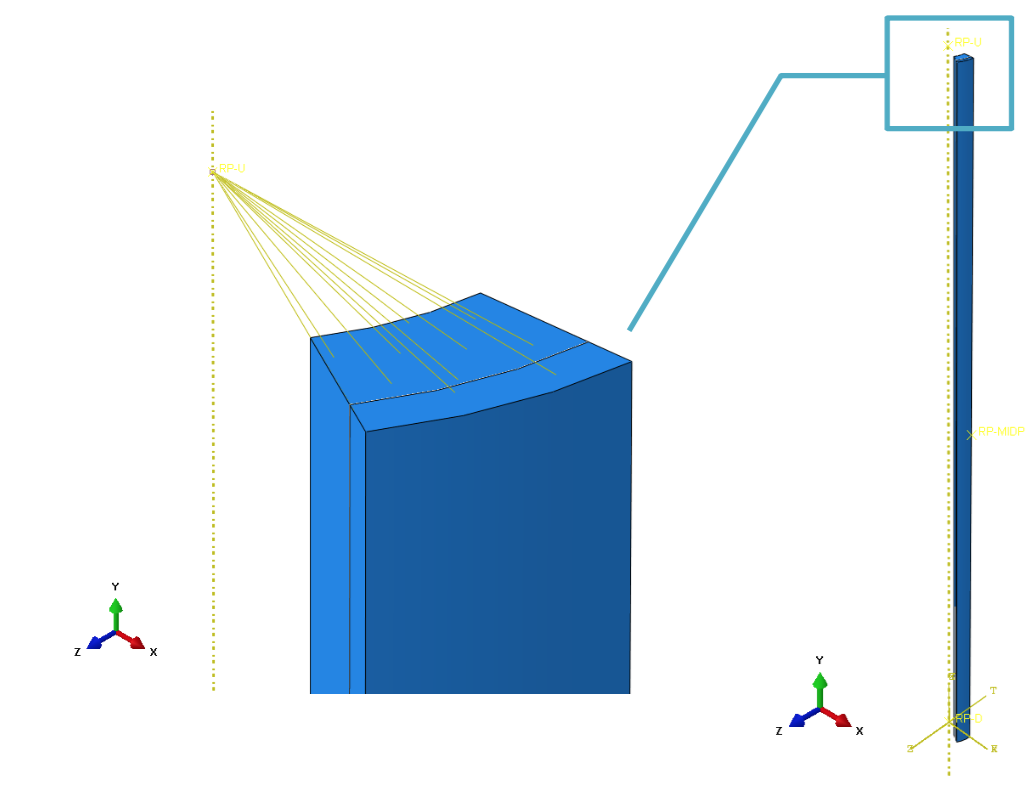
\includegraphics[width=0.3\linewidth]{figure/chap3/FEM/periodic-sym-2}
	\label{fig:periodic-sym-2}
}
\subfigure[周期对称模型]{
	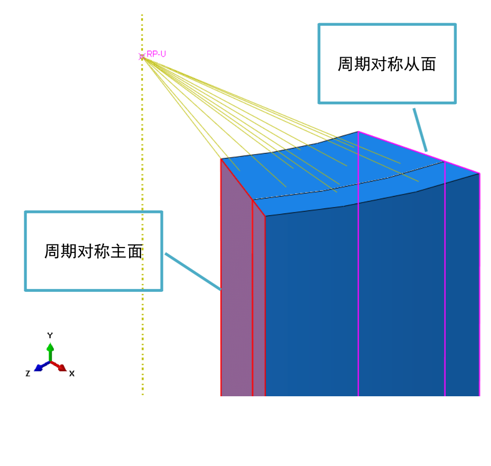
\includegraphics[width=0.2\linewidth]{figure/chap3/FEM/periodic-sym}
	\label{fig:periodic-sym-3}
}
\fcaption{几何模型简化}{Geometry Simplification}
\end{figure*}





而在软管施加内压荷载的有限元模型中,建立完整的模型的方法更为通用。建立的模型如图\ref{fig:whole-m-2}所示。模型中内管与编织层之间为Tie接触(完全粘连,不发生相对位移),因为金属纤维的编织层再生产时会施加预紧力,金属纤维会在质地相对较软的内管形成较深的压痕,内管和编织层很难发生相对滑动。

\begin{figure*}[!htp]
\centering
\subfigure[接触关系]{
	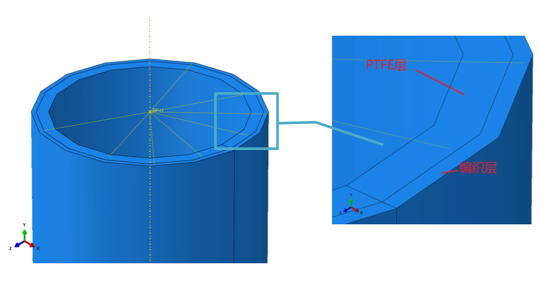
\includegraphics[width=0.45\linewidth]{figure/chap3/FEM/whole-m}
}
\hspace{0.5cm}
\subfigure[荷载施加]{
	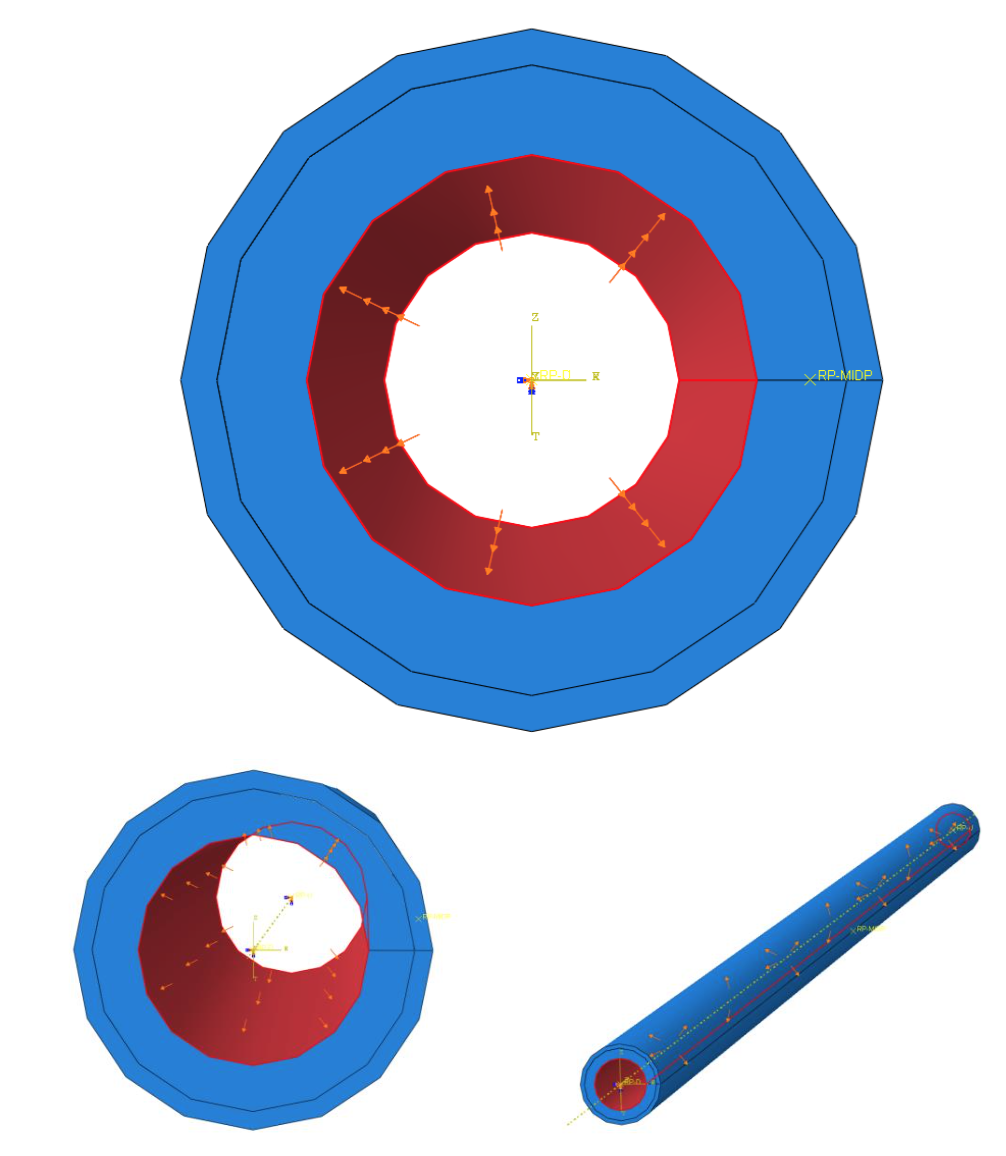
\includegraphics[width=0.25\linewidth]{figure/chap3/FEM/whole-m-2}
}
\fcaption{完整模型}{Full FEM Model}
\label{fig:whole-m-2}
\end{figure*}

但是值得注意的是,非金属纤维由于纤维直径较小,不容易在内管上产生压痕,因此很容易发生相对滑动。有限元针对非金属纤维编织层建模时需要考虑这种接触关系的影响。

\subsection{仿真结果}

简化几何模型,建立有限元模型,并导入\uma 子程序接口后,\aba 就能进行自定义本构模型的求解了。有限元结果大致如\ref{fig:results-2}所示,具体的数值分析,以及针对仿真结果进行的理论修正,将在后面的章节进行介绍。
\begin{figure*}[!htp]
\centering
\subfigure{
	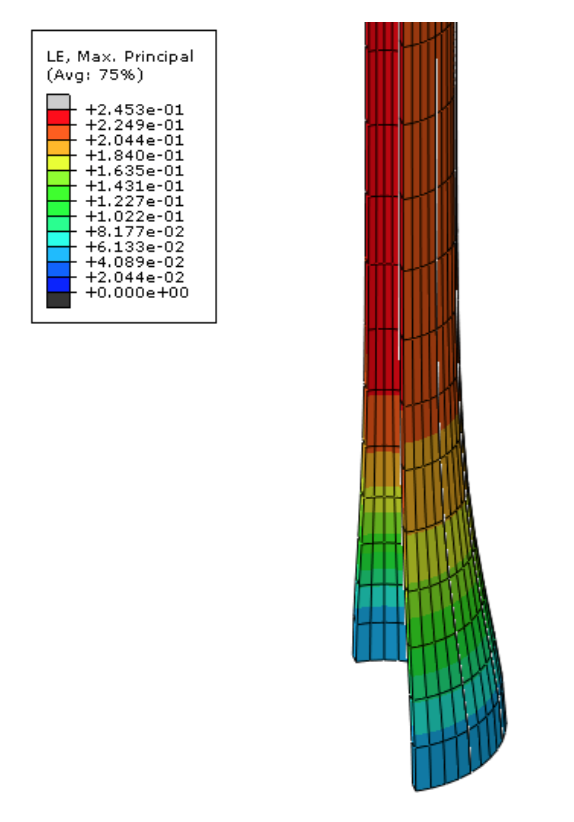
\includegraphics[width=0.3\linewidth]{figure/chap3/FEM/results}
}
\hspace{0.5cm}
\subfigure{
	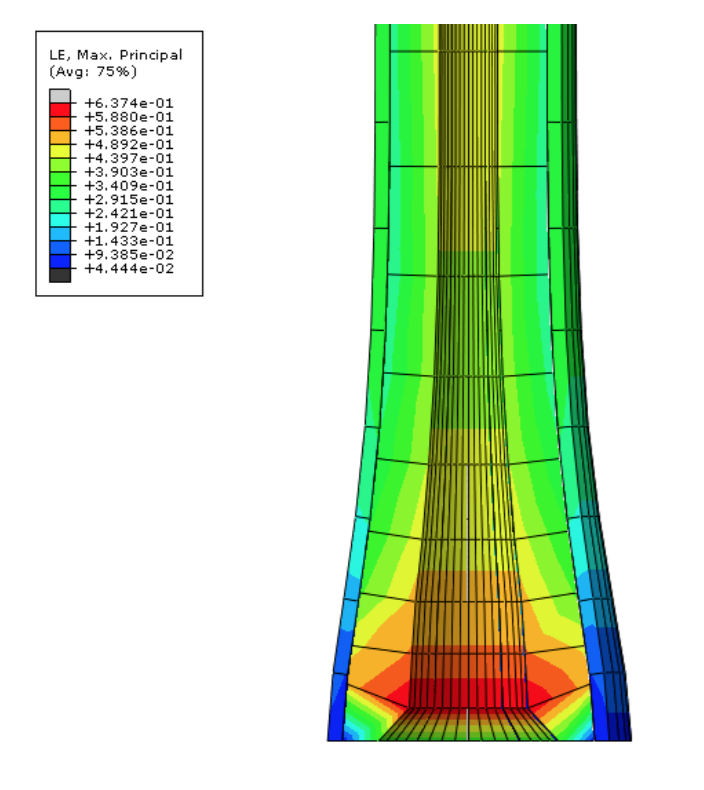
\includegraphics[width=0.38\linewidth]{figure/chap3/FEM/results-2}
}
\fcaption{仿真结果}{FEM Simulation Results}
\label{fig:results-2}
\end{figure*}


\section{小 ~ 结}

本章主要总结介绍了\ha 对于编织加强层提出的理论,给出了具体的理论推导过程。明确了该理论的框架,包括了3条基本假设,编织角理论,以及平均化刚度矩阵理论。编织角理论体现了钢绞线理论的内核,反映了编织层在拉伸过程中的“几何非线性”;刚度矩阵理论基于对特征单元的分析,但\ha 并没有进行深入的研究。

本章还讨论了\ha 在其拉伸试验中提出的“锁定叫假设”,而该假设将作为本研究试验的一个需要重点关注的对象。

此外,本章还对该理论体系下的仿真方法进行了探索,介绍了基于\uma 二次开发本构关系的方法。



